\input{../YKY-preamble.tex}
% \usepackage[no-math]{fontspec}
% \setmainfont[BoldFont=Alibaba_Sans_Regular.otf,ItalicFont=Alibaba_Sans_Light_Italic.otf]{Alibaba_Sans_Light.otf}

\usepackage[backend=biber]{biblatex}
\bibliography{../AGI-book}

\usepackage[active,tightpage]{preview}		% for continuous page(s)
\renewcommand{\PreviewBorder}{0.5cm}
\renewcommand{\thempfootnote}{\arabic{mpfootnote}}

\usepackage[absolute,overlay]{textpos}		% for page number on upper left corner

\usepackage{color}
% \usepackage{mathtools}
\usepackage[hyperfootnotes=false]{hyperref}

% \usepackage[backend=biber,style=numeric]{biblatex}
% \bibliography{../AGI-book}
% \renewcommand*{\bibfont}{\footnotesize}

\usetikzlibrary{shapes}
% \usepackage[export]{adjustbox}	% ??
\usepackage{verbatim} % for comments
% \usepackage{newtxtext,newtxmath}	% Times New Roman font

% \titleformat{\subsection}[hang]{\bfseries\large\color{blue}}{}{0pt}{} 
% \numberwithin{equation}{subsection}

\newcommand{\underdash}[1]{%
	\tikz[baseline=(toUnderline.base)]{
		\node[inner sep=1pt,outer sep=10pt] (toUnderline) {#1};
		\draw[dashed] ([yshift=-0pt]toUnderline.south west) -- ([yshift=-0pt]toUnderline.south east);
	}%
}%

\newcommand{\witness}{\scalebox{0.9}{$\blacksquare$}}
\newcommand\reduline{\bgroup\markoverwith{\textcolor{red}{\rule[-0.5ex]{2pt}{0.4pt}}}\ULon}

%\DeclareSymbolFont{symbolsC}{U}{txsyc}{m}{n}
%\DeclareMathSymbol{\strictif}{\mathrel}{symbolsC}{74}
%\DeclareSymbolFont{AMSb}{U}{msb}{m}{n}
%\DeclareSymbolFontAlphabet{\mathbb}{AMSb}
%\setmathfont{lmroman17-regular.otf}
\DeclareMathOperator*{\argmin}{arg\,min}
\DeclareMathOperator*{\argmax}{arg\,max}

% \usepackage[most]{tcolorbox}
%\tcbset{on line, 
%	boxsep=4pt, left=0pt,right=0pt,top=0pt,bottom=0pt,
%	colframe=red,colback=pink,
%	highlight math style={enhanced}
%}
%\newcommand{\atom}{\vcenter{\hbox{\tcbox{....}}}}

\let\oldtextbf\textbf
\renewcommand{\textbf}[1]{\textcolor{blue}{\oldtextbf{#1}}}

\newcommand{\logic}[1]{{\color{violet}{\textit{#1}}}}
\newcommand{\underconst}{\includegraphics[scale=0.5]{../2020/UnderConst.png}}
\newcommand{\KBsymbol}{\vcenter{\hbox{\includegraphics[scale=1]{../KB-symbol.png}}}}
\newcommand{\token}{\vcenter{\hbox{\includegraphics[scale=1]{token.png}}}}
\newcommand{\proposition}{\vcenter{\hbox{\includegraphics[scale=0.8]{proposition.png}}}}

\begin{document}
	
\begin{preview}

\title{\vspace{-1.5cm} \bfseries\color{blue}{\LARGE AGI from the perspective of\\
		categorical logic}}

\author{YKY} % Your name
% \date{\vspace{-2cm}} % Date, can be changed to a custom date

\maketitle

\setcounter{section}{-1}
\newcounter{mypage}
\setcounter{mypage}{0}

% (1) Circled page number on upper left corner
\begin{textblock*}{5cm}(2.1cm,2.3cm) % {block width} (coords) 
	{\color{red}{\large \textcircled{\small \themypage}}}
	\addtocounter{mypage}{1}
\end{textblock*}

\begin{minipage}{\textwidth}
	\setlength{\parskip}{0.4\baselineskip}
			
\section{Basics}

\begin{itemize}
\cc{	\item 首先 范畴逻辑 的中心思想是 Curry-Howard isomorphism,不明白这点无从入门。
}{
\item The starting point of categorical logic is really the \textbf{Curry-Howard isomorphism}, without which you won't be able to understand the sequel.
}
\cc{	\item Curry-Howard 同构 指的是: 用数学上 函数的	模拟 逻辑上的蕴函关系 $A \Rightarrow B$.
}{
\item Curry-Howard correspondence is the idea of using a mathematical \textbf{function} $f: A \rightarrow B$ to simulate or implement the process of logic deduction, specifically $A \Rightarrow B$.
}
\cc{	\item 由于这个对应关系,逻辑上的 命题 A 对应与函数的 domain A.  也就是说,命题对应于某种类似 \textbf{空间} 的东西。
}{
\item From this perspective, a logic \textbf{proposition} $A$ corresponds to the \textbf{domain} $A$ of a function.  That is, a proposition is akin to something like a \textbf{space}.
}
\cc{	\item 而那空间里的物体,就是所谓 proof objects,即该命题的证明。
}{
\item Objects in that space are so-called \textbf{proof objects}, we use $\witness$ to denote them.
}
\cc{	\item 这样说有点难懂,但其实我们天天都面对这种东西:那就是 神经网络。
}{
\item It may take a while to get used to, but in fact we see this idea in use almost every day: in \textbf{neural networks}.
}
\cc{	\item 它将某些 向量 映射到 别的向量,向量 就是 proof,
}{
\item A neural network maps certain vectors to vectors. Each vector is a proof.
}
\cc{	\item 某个向量周围的空间(在一定误差下)表示 同一概念,所以不妨把那邻域的空间看成是一个 逻辑命题。
}{
\item The space near a positional vector (under some error margin) ought to represent the \textbf{same} concept.  So we might as well think of the neighborhood space as a logical proposition.
}
\cc{	\item 这种做法实在太明显也太自然了。
}{
\item This way of doing things is really very obvious and natural.
}
\end{itemize}

\cc{做了这个对应之后,逻辑上 $A \Rightarrow B$ 的真值表,很奇妙地跟函数空间的基数 (cardinality) 吻合:
}{
One evidence that this correspondence is on the right track is the truth table of $A \Rightarrow B$, which perfectly matches the cardinalities of the function spaces:
}
\begin{equation}
\label{truth-table:material-implication}
\begin{tabular}{|c|c|c|c|}
\hline 
$A$ & $B$ & $A \Rightarrow B$ & $B^A$ \\ 
\hline \hline 
0 & 0 & 1 & $0^0 = 1$ \\
\hline 
0 & 1 & 1 & $1^0 = 1$ \\ 
\hline 
1 & 0 & 0 & $0^1 = 0$ \\ 
\hline 
1 & 1 & 1 & $1^1 = 1$ \\ 
\hline 
\end{tabular} 
\end{equation}

\cc{这也让我们更有信心,Curry-Howard 同构是将逻辑 数学化 的正确方向。
}{
}

\cc{范畴逻辑 的目的就是:利用范畴论里各种抽象的工具,描述 逻辑的结构。
}{
The goal of categorical logic is to use categorical tools as much as possible, to \textbf{describe} the structure of logic.
}

\begin{itemize}

\cc{\item 基于 命题 = 某种空间,那么 很自然地,我们可以用范畴里的 物体 (objects) 代表命题,这种做法更为一般。
}{
	\item ``Propositions = some kind of spaces'' generalizes naturally in category theory to ``propositions = \textbf{objects} in a category''.
}

\cc{\item 用范畴论 里的 products 表达逻辑上的 $\wedge$ 或 $\vee$,exponentiation 表达 逻辑上的 $A \Rightarrow B$,这也同时是范畴里的 morphism $A \rightarrow B$.
}{
	\item We use \textbf{products} in category theory to express logic $\wedge$ and $\vee$, and \textbf{exponentiations} $B^A$ for $A \Rightarrow B$.  The latter are also \textbf{morphisms} $A \rightarrow B$ in the category.
}

\cc{\item $\forall$ 和 $\exists$ 是 某种 variable substitution map 的 adjoint,因为 adjunction 也是数学上常见的结构:
}{
	\item $\forall$ and $\exists$ are described as \textbf{adjoints} to certain variable-substitution maps.  For example in $\forall x. \phi(x,y) $ the quantifier $\forall x$ projects the space of $(x,y)$ down to $(y)$ only, so the resulting expression is no longer about $x$.
}
\begin{equation}
\vcenter{\hbox{\includegraphics[scale=0.8]{../2020/Lawvere-cylindrification-forall.png}}}
\quad
\vcenter{\hbox{\includegraphics[scale=0.8]{../2020/Lawvere-cylindrification-exists.png}}}
\end{equation}
\cc{(这比较复杂,但我以前也讲解过了,重要的是理解整体的概念,暂时不要迷失在细节里)
}{
	(This part is a bit complicated, but I have explained it elsewhere. The important thing is to understand the overall concept and not get lost in the details just yet)
}
\end{itemize}

\end{minipage}
\end{preview}

\begin{preview}
\begin{textblock*}{5cm}(2.1cm,2.3cm) % {block width} (coords) 
	{\color{red}{\large \textcircled{\small \themypage}}}
	\addtocounter{mypage}{1}
\end{textblock*}

\begin{minipage}{\textwidth}
	\setlength{\parskip}{0.4\baselineskip}

\section{Where is GPT?}

\cc{逻辑 谓词 (predicates) 表示为 纤维结构 (fibration), 即以一个 base 空间 对某个上层空间做 ``indexing,'' 可以看下图理解:
}{
Logic \textbf{predicates} are described as \textbf{fibrations}, that is, an upper space ``indexed'' by the base space:
}
\begin{equation}
\vcenter{\hbox{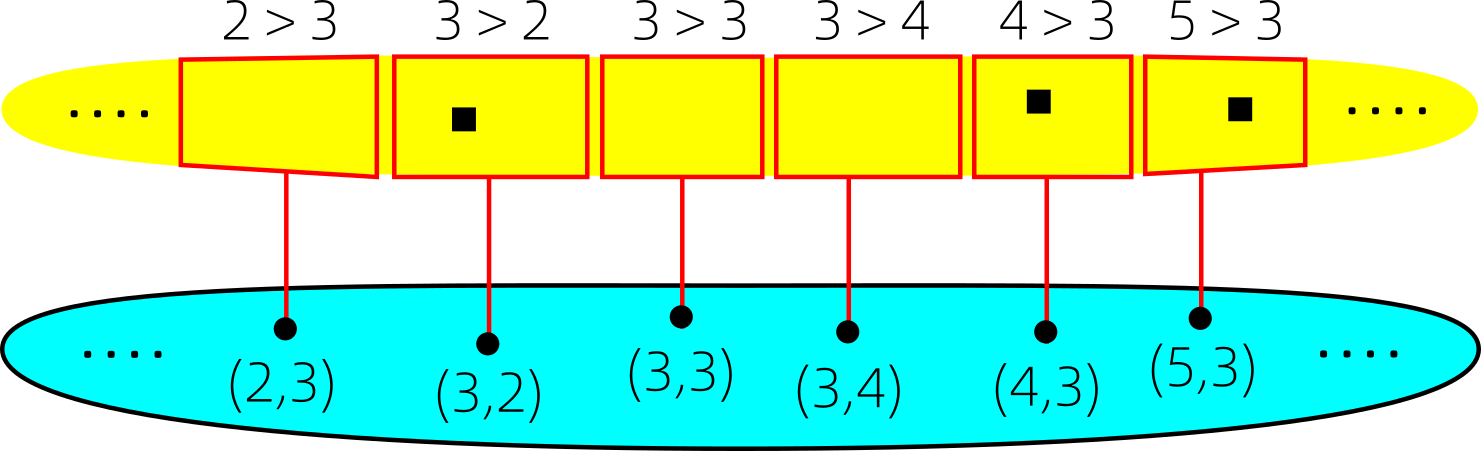
\includegraphics[scale=0.6]{sheaf-of-propositions-over-numbers.png}}}
\end{equation}

\cc{我们考虑的是某个二元关系 ``$>$'', 所以底层 base space 是 $\mathbb{N} \times \mathbb{N}$ 即一对对的自然数。 我们可以构成 谓词逻辑命题 $>(a,b)$,而因为 Curry-Howard,这些命题是一些 “空间”,即上层那些黄色的方格。 每个方格是一个命题,它可以有或没有 证明,即黑色的小方格 $\witness$.
}{
Here we are considering the binary relation ``$>$'', so the indexing space consists of pairs of natural numbers $\mathbb{N} \times \mathbb{N}$.  We can form relational propositions $>(a,b)$, and because of Curry-Howard, these propositions are ``spaces'', ie, yellow squares above.  Each square is a proposition, which may or may not have a proof ($\witness$).
}

\cc{上面 所有黄色方格的 并集 就是一个 层 (sheaf),它是所有命题的空间 $\mathbb{L}$. GPT 就是一个将 命题 映射到 命题 的 逻辑推论算子 (logic consequence operator). 但注意: GPT 是一种 set-valued mapping, 它作为函数的 domain 不是 $\mathbb{L}$,而是 命题的 集合 的空间,亦即 power set of L 或者可以记作 PL:
}{
The union of all the yellow squares above is a \textbf{sheaf}, which is the space $\mathbb{L}$ of propositions.  \textbf{GPT} is a \textbf{logic consequence operator} that maps propositions to propositions.  But note:  GPT is a \textbf{set-valued map}.  Its domain is not $\mathbb{L}$ but the the power set $2^\mathbb{L}$ or $\mathcal{P}(\mathbb{L})$:
}
\begin{equation}
\vcenter{\hbox{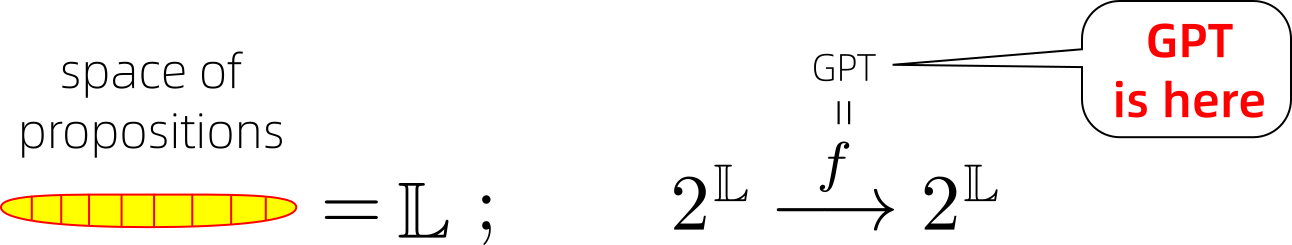
\includegraphics[scale=0.9]{GPT-is-here.png}}}
\end{equation}

\cc{大家知道了「GPT 在哪里」,是不是觉得清晰了很多? 至少我是这样觉得的,因为我非常熟悉 logic-based AI, 我习惯了从这个角度 理解我需要用的数学。
}{
Knowing where GPT fits into the scheme of things, provides some clarity.  At least for me, because I'm very familiar with \textbf{logic-based AI}, I tend to understand the mathematics from this perspective.
}

\end{minipage}
\end{preview}

\begin{preview}
\begin{textblock*}{5cm}(2.1cm,2.3cm) % {block width} (coords) 
{\color{red}{\large \textcircled{\small \themypage}}}
\addtocounter{mypage}{1}
\end{textblock*}

\begin{minipage}{\textwidth}
\setlength{\parskip}{0.4\baselineskip}

\section{What is HoTT?}

\cc{由于 Curry-Howard 说 命题 是 某种「空间」,那么这空间会不会有 拓扑结构? 最近英年早逝的天才 Voevodsky 提出了 命题空间内有 homotopy 的结构,那就是 HoTT (homotopy type theory) 的基本思路。
}{
As Curry-Howard suggest that propositions are some kind of ``spaces'', can they have topological structure?  This is the original idea of \textbf{HoTT} (homotopy type theory) proposed by Voevodsky.
}
\begin{equation}
\vcenter{\hbox{\includegraphics[scale=0.4]{../2020/Voevodsky.jpg}}} \nonumber
\end{equation}

\cc{以我肤浅的理解,一个命题 要么有证明 或没有证明,如果有证明的话,A 证明和 B 证明 是没有分别的。 但 HoTT 提出 它们可以有区别。 在一个命题的内部空间里,path-connected 的两个点 (proofs) 被视为 identical,但这空间内可以有不是 path-connected 的空间结构,那么 两个 proofs 就可以视为 不相同。
}{
From my limited understanding, a proposition either has a proof or not have a proof. If there is a proof, there is no difference between one proof or another.  But HoTT posits that they can differ. In the internal space of a proposition, two \textbf{path-connected} points (proofs) are regarded as identical, but there can be regions that are not path-connected in this space, so their proofs are regarded as different.
}

\cc{一个例子是: 西方古代将 金星 视为 morning star 和 evening star,而不知道它们其实是同一颗星。 这就是 intension 和 extension 的不同(意指和实际的外延不同),涉及 内涵逻辑 (intensional logic) 的问题,它的 语义可以用 模态逻辑 (modal logic) 和 Montague semantics 处理,详细可参看这篇文章: https://plato.stanford.edu/entries/logic-intensional/ 
}{
An example:  The ancients regarded Venus as the Morning Star and Evening Star, without knowing that they were actually the same star. This is the difference between intension and extension, which can be handled by \textbf{intensional logic}, and can be formulated using \textbf{modal logic} and Montague semantics. For details, see this article: \href{https://plato.stanford.edu/entries/logic-intensional/}{https://plato.stanford.edu/entries/logic-intensional/}
}
\begin{equation}
\vcenter{\hbox{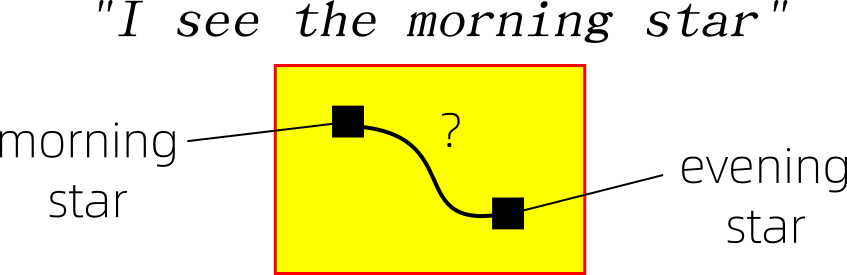
\includegraphics[scale=0.8]{morning-star.png}}}
\end{equation}

\cc{又例如 同一个群 可以有不同的 群展示 (group presentations),似乎也可以用 HoTT 处理。
}{
For another example, a group can have different \textbf{group presentations}, a situation that seems applicable by HoTT.
}

\cc{这些 不是 path-connected 的空间 具有 groupoid 结构,可以产生 1-groupoid,2-groupoid 等不同的层级,直至 ∞-groupoid. 这方面我暂时不太理解。
}{
These spaces that are not path-connected have a \textbf{groupoid} structure, with multiple levels such as 1-groupoid, 2-groupoid, ... up to $\infty$-groupoid.  I am not familiar with these aspects.
}

\cc{大家可以看到,HoTT 涉及的是「真」的 内部(即黄色方格),但 AGI 主要涉及的是 逻辑的应用,是在 命题空间的 外部(即整个黄色香蕉那空间、其子集空间 之间的映射)。
}{
As the reader can see, HoTT is concerned with the interior of ``truth'' (ie, the yellow square), but AGI is mainly concerned with \textbf{inference}, which acts on the proposition space (ie, the entire yellow ``banana'' space).
}

\cc{这并不是说 HoTT 对 AGI 没用,但它的影响是比较 微妙 (subtle) 的,我暂时不能判断。
}{
This is not to say that HoTT is useless for AGI, but its impact is subtle and I cannot judge it yet.
}

\cc{其实 Transformer 有能力学习非常复杂的 syntactic manipulations,也就是说,它可以隐式地学习各种我们研究的逻辑,例如 modal logic,的推导方式。 如果这样,它似乎可以「绕过」而不需要我们直接 implement 那些麻烦的逻辑形式。 但也有可能是,我们人工地 附加某些 逻辑结构 的 约束,可以加速 深度学习。 这些需要实验证实,是现时非常重要的方向。
}{
In fact, the \textbf{Transformer} has the ability to learn very complex syntactic manipulations, that is, it can implicitly learn the derivation steps of various logics such as modal logic.  If so, it seems that we be ``bypassed'' various special logics without the need to explicitly implement them.  But it is also plausible that we by imposing certain logical structural constraints that we can accelerate deep learning. These need to be verified experimentally and are promising research directions.
}

\end{minipage}
\end{preview}

\begin{preview}
\begin{textblock*}{5cm}(2.1cm,2.3cm) % {block width} (coords) 
	{\color{red}{\large \textcircled{\small \themypage}}}
	\addtocounter{mypage}{1}
\end{textblock*}

\begin{minipage}{\textwidth}
	\setlength{\parskip}{0.4\baselineskip}

\section{Modal logic and possible worlds}

\cc{模态逻辑 (modal logic) 与 可能世界语义 (possible world semantics) 是一种很 powerful 的逻辑形式,它可以处理很多哲学逻辑上的课题。 以前我学习符号逻辑 AI 时,比较忽略它,因为要在 计算机上实现 模态逻辑引擎 比较麻烦。  随着 AGI 越来越接近,我觉得有必要更仔细研究一下。
}{
Modal logic and possible world semantics are very powerful forms of logic that can handle many problems in philosophical logic.  When I studied symbolic logic AI in the past, I mostly ignored it because it was troublesome to implement a modal logic engine on a computer.  As AGI gets closer to reality, I feel the need to take a closer look to modal logics.
}

\cc{这篇文章的重点是:模态逻辑 具有 层 (sheaf) 和 topos 的结构。 事实上,topos semantics 是逻辑语义学的 「最新」 发展 (其实也很旧了 哈),有说 topos 语义能处理几乎所有我们知道的逻辑语义(究竟有什么例外我也不知)。
}{
The main point of this section is: modal logic has a structure of sheaves and toposes.  Topos semantics is the ``latest'' development of logical semantics (it's actually quite old, haha). It is said that topos semantics can handle almost all the logical semantics we know (though I don't even know what are the exceptions).
}

\cc{以下这个图就是精要: 
}{
The basic picture is this:
}
\begin{equation}
\vcenter{\hbox{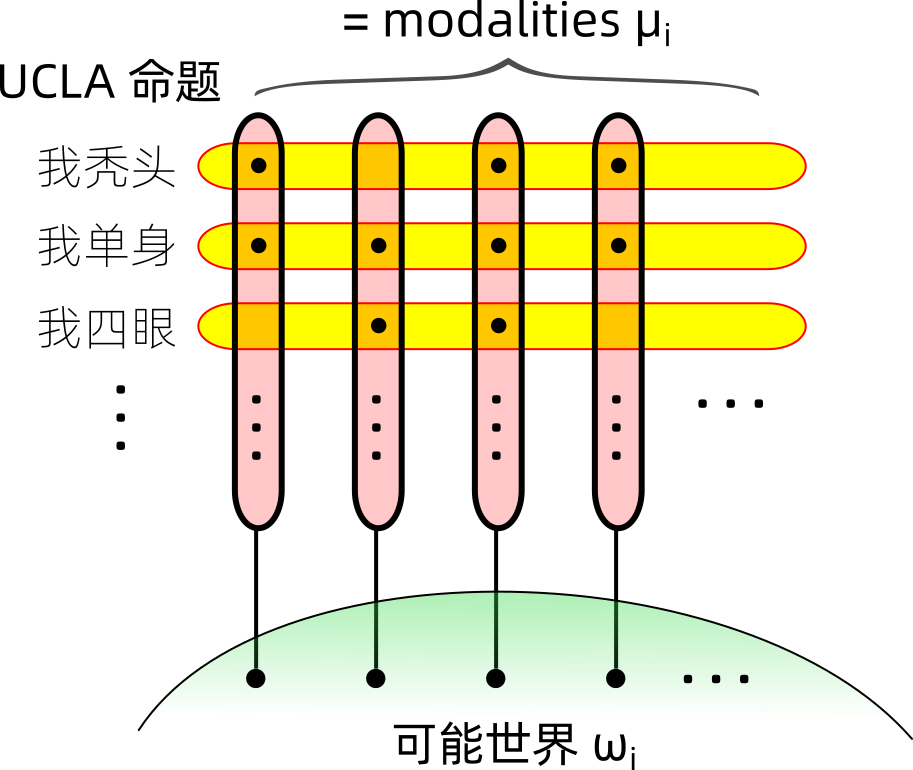
\includegraphics[scale=0.7]{possible-worlds-as-sheaf.png}}}
\end{equation}

\begin{itemize}
\cc{	\item 底下的绿色集合 纯粹是 每个可能世界的指标 (index), 例如 $ \mathbb{N} = \{ 1,2,3,4 \} $
}{
 \item The green set underneath are just \textbf{indexes} to each possible world, for example $ \mathbb{N} = \{ 1,2,3,4 \}$
}
\cc{	\item 每个蓝色的「冰条」代表一个 可能世界。 它们构成一个 纤维结构 (fibration) 或 层。
}{
\item Each red ``\textbf{stalk}'' represents a possible world.  They form a \textbf{fibration} over the base.
}
\cc{	\item 红色横线 表示 每个逻辑命题 在不同的可能世界内的取值情况
}{
\item The yellow horizontal bars show the state of truth of each logic \textbf{proposition} for each possible world.
}
\cc{	\item Modality = 可能世界 的同义词,在 John L Bell 的书里用这术语
}{
\item \textbf{Modality} = synonym for possible world, a terminology used in John L Bell's book
}
\end{itemize}

\cc{但我觉得最精简的论述是这篇 2008 的论文: Topology and Modality: The Topological Interpretation of First-Order Modal Logic by Awodey \& Kishida.  本文主要是基于这篇。
}{
This basic structure is laid out in the paper: \textit{Topology and Modality: The Topological Interpretation of First-Order Modal Logic} by [Awodey \& Kishida 2008].
}

\cc{那篇论文的重点是: modal propositional logic 有某种简单的 拓扑语义,而 first-order predicate logic 有另一种 denotational 语义,将两者「乘积」起来,构成 first-order modal logic 的 sheaf 语义。(学过 编程语言语义学 的人可能已听过 denotational semantics.) 我们先分别介绍这两种语义:
}{
The key point of that paper is: modal propositional logic has some simple topological semantics, and first-order predicate logic has another kind of denotational semantics. The "product" of the two constitutes the sheaf semantics of first-order modal logic. (Those who have studied programming language semantics may have heard of denotational semantics.) Let’s first introduce these two semantics respectively:
}

\subsection{\cc{模态逻辑的拓扑语义}{Topological semantics of modal logic}}

\cc{这是 Tarski-McKinsey 1944年 最先提出的。 想法就是:
}{
This was first proposed by Tarski-McKinsey in 1944. The idea is:
}

\begin{itemize}
\cc{	\item 一个 可能世界 对应于 拓扑空间的一个 开集 (open set)
}{
\item A possible world corresponds to an open set of topological space (open set)
}
\cc{	\item 一个 命题 等同于 其所在为真的可能世界的 集合 (= set of open sets) \\
}{
\item A proposition is equivalent to the set of possible worlds in which it is true (= set of open sets) \\
}
\cc{		这种命题称为「UCLA 命题」,由加州大学的研究者们提出
}{
This proposition is called the "UCLA proposition" and was proposed by researchers at the University of California
}
\cc{	\item 模态算符 ⋄ 和 ◻ 分别对应于拓扑上的 closure 和 interior operation
}{
\item Modal operators ⋄ and ◻ correspond to topological closure and interior operations respectively.
}
\end{itemize}

\cc{举例来说,只考虑下面 4个可能世界,那么「我破脚」并不是必然的,但「我单身」是必然的。「◻ 我单身」这命题的 interior = 全域,所以命题为 真。
}{
For example, if we only consider the following four possible worlds, then "I have a broken foot" is not inevitable, but "I am single" is inevitable. The proposition "◻ I am single" has interior = the whole domain, so the proposition is true.
}

\begin{equation}
\vcenter{\hbox{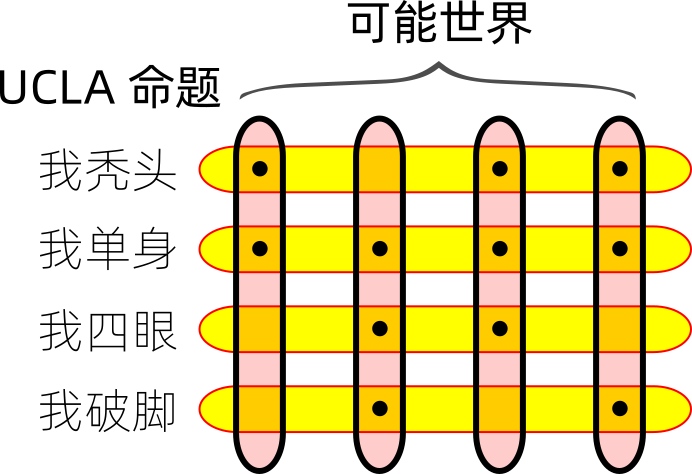
\includegraphics[scale=0.7]{possible-worlds-example.png}}}
\end{equation}

\subsection{\cc{谓词逻辑的 denotational 语义}{Denotational semantics of predicate logic}}

\cc{这部分是比较经典的 模型论 (model theory),我不想花太多时间解释,基本上它用一个 结构  来 诠释 (interpret) 逻辑命题。D 是一个逻辑物体的 论域 (domain),例如 { 苹果,香蕉,橙,John,Mary } 等。 R 是一些 关系 (relations) 或 谓词 (predicates),例如「x 是男人」、「x 喜欢吃 y」等。 f 是一些 函数 (functions),例如「x 的妈妈」、「x 最喜欢的水果 」、等。 c 是一些 常数,例如「c1 = John」等。 一个结构 M 包含足够的资料去 赋值 (interpret) 任何命题的真假。 也可以把 M 看成一个 可能世界 的资料,只是它是唯一的世界而已。
}{
This part is the more classic model theory. I don’t want to spend too much time explaining it. Basically, it uses a structure to interpret logical propositions. D is the domain of a logical object, such as {apple, banana, orange, John, Mary}, etc. R is some relations or predicates, such as "x is a man", "x likes to eat y", etc. f is some functions, such as "x's mother", "x's favorite fruit", etc. c is some constant, such as "c1 = John" etc. A structure M contains enough information to interpret the truth or falsity of any proposition. M can also be regarded as the data of a possible world, but it is the only world.
}
\begin{equation}
\vcenter{\hbox{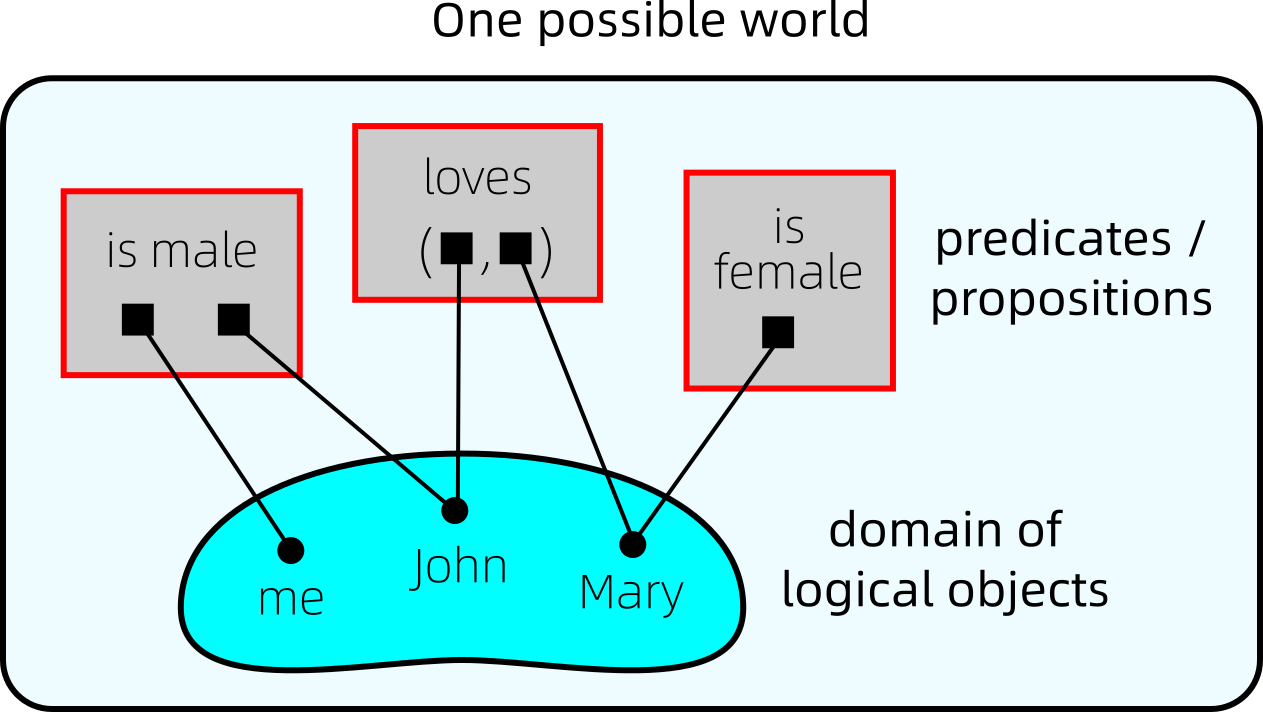
\includegraphics[scale=0.7]{possible-world-single-example.png}}}
\end{equation}

\end{minipage}
\end{preview}

\begin{preview}
\begin{textblock*}{5cm}(2.1cm,2.3cm) % {block width} (coords) 
{\color{red}{\large \textcircled{\small \themypage}}}
\addtocounter{mypage}{1}
\end{textblock*}

\begin{minipage}{\textwidth}
\setlength{\parskip}{0.4\baselineskip}

\section{Sheaf semantics}

\cc{所谓结合,似乎是一种乘积,或者更简单地就是 将纤维顺着方向并排起来,这是一个 加法:
}{
The so-called combination seems to be a product, or more simply, lining up the fibers in the direction, which is an addition:
}

\cc{构成一个 sheaf,而 sheaf 也可以看成是 topos.  整体的图像大概是这样的:
}{
Form a sheaf, and sheaf can also be regarded as topos. The overall image is roughly like this:
}
\begin{equation}
\vcenter{\hbox{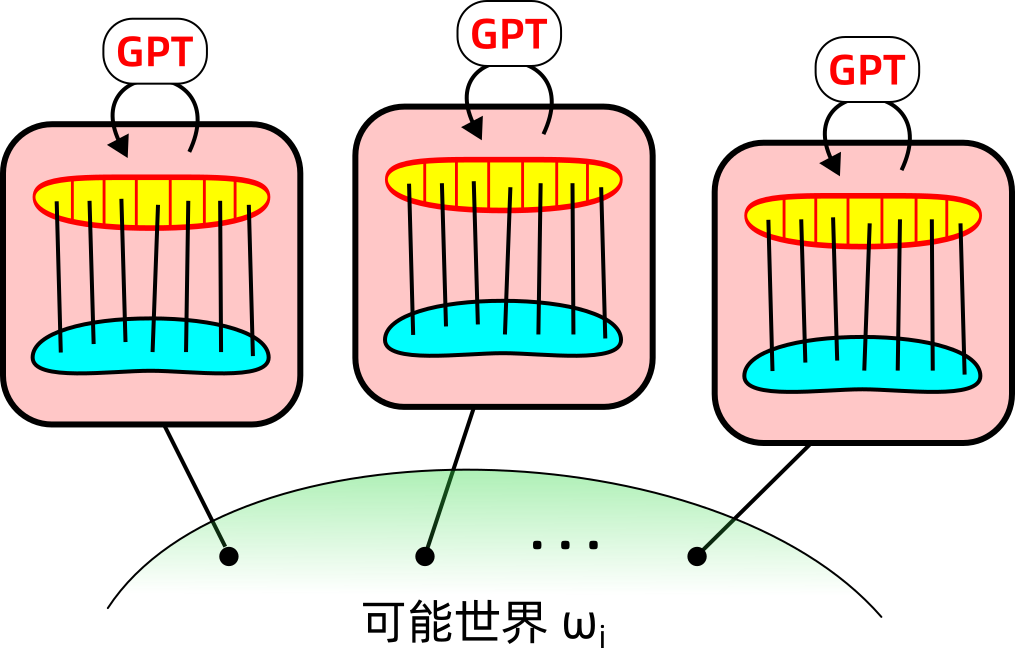
\includegraphics[scale=0.7]{possible-worlds-as-sheaf-with-GPT.png}}}
\end{equation}

\begin{itemize}
\cc{	\item 从 人脑 的角度看,它处理「可能世界」的能力是很有限的。 
}{
\item From the perspective of the human brain, its ability to process "possible worlds" is very limited.
}
\cc{	\item 最经典的例子是 下棋 时,每个预测的棋步就是一个可能世界。 在一般情况下,人们通常只能预测 3-5 步。
}{
\item The most classic example is when playing chess, each predicted move is a possible world. In general, people can usually predict only 3-5 moves.
}
\cc{	\item 每个 可能世界 其实跟当前的世界 只相差一个命题,似乎在实践上不必把可能世界想象成「庞然大物」。
}{
\item Each possible world is actually only one proposition different from the current world. It seems that in practice, there is no need to imagine possible worlds as "monsters".
}
\cc{	\item 可能世界 是在思考时 动态地 (dynamically) 产生的,我们不可能快速地 根据每个可能世界 训练一个 GPT,因此上面的 GPT's 是同一个训练结果的 拷贝。
}{
\item Possible worlds are generated dynamically when thinking. We cannot quickly train a GPT according to every possible world, so the above GPT's are copies of the same training results.
}
\cc{	\item 如要实现 模态逻辑 推理,要将上面那个「小 GPT」的功能扩充,让它可以处理多个可能世界的推理。暂时我想到的方法,纯粹是沿用 经典逻辑 AI 的思路,例如将每个可能世界 tag 上特定的命题,然后再计算
}{
\item If you want to implement modal logic reasoning, you need to expand the function of the "little GPT" above so that it can handle reasoning in multiple possible worlds. The method I think of for the time being is purely to follow the idea of ​​classic logical AI, such as tagging each possible world with a specific proposition, and then calculating
}
\cc{	\item 当可能世界的个数很少时,拓扑 的 closure / interior 概念似乎没有太大的启发性。从 计算机 的角度看,连续空间是很「理想化」的东西,实际上很难实现。
}{
\item When the number of possible worlds is small, the concept of topological closure / interior does not seem to be very enlightening. From a computer point of view, continuous space is very "ideal" and is actually very difficult to achieve.
}

\end{itemize}

\cc{这些都算颇直观的,我有空会详细一点看,但现在突然觉得这个方向未必太有用....
}{
These are quite intuitive. I will look at them in detail when I have time, but now I suddenly feel that this direction may not be too useful...
}

\subsection{Some technical details on sheaves}

\end{minipage}
\end{preview}

\begin{preview}
\begin{textblock*}{5cm}(2.1cm,2.3cm) % {block width} (coords) 
	{\color{red}{\large \textcircled{\small \themypage}}}
	\addtocounter{mypage}{1}
\end{textblock*}
	
\begin{minipage}{\textwidth}
	\setlength{\parskip}{0.4\baselineskip}
		
\section{What's the use of all these to AGI?}

		
\end{minipage}
\end{preview}

\end{document}
